\pdfminorversion=5
\pdfobjcompresslevel=2
\documentclass[english]{article}

%%
% For revision notes only - not needed in final version
\usepackage{changes}
\definechangesauthor[Nathan West]{nw}{orange}
\definechangesauthor[Doug Geiger]{dg}{red}
%%

%\usepackage[T1]{fontenc}
\usepackage{units}
\usepackage{courier}
\usepackage[pdftex]{graphicx}
\usepackage{mcite}
\usepackage{todonotes}
\usepackage{hyperref}
\usepackage{ifpdf}
\usepackage{listings}
\usepackage{authblk}
\ifpdf
\hypersetup{
 pdfauthor={Nathan West},
 pdftitle={Benchmarking GNURadio on Various General Purpose Processing Architectures},
 pdfborderstyle={/S/U/W1}
}
\fi

\author[1]{Nathan West}
\author[1]{Douglas Geiger}
\author[2]{George Scheets}
\affil[1]{US Naval Research Laboratory}
\affil[2]{Oklahoma State University}
\title{Benchmarking GNU Radio Kernels and Multi-Processor Scheduling}

\graphicspath{{../images/}}

\begin{document}
\maketitle

\abstract{%
The growth of Software Defined Radio (SDR) using general purpose processors (GPPs) brings a new engineering decision of processor selection to radio design.
Processor selection is an important engineering decision that affects size, weight, power, and data throughput of a SDR. 
We approach the problem by benchmarking a variety of general-purpose processors using the GNU Radio framework. 
We present a methodology of benchmarking for SDR, an integrated set of tools for benchmarking, and results from select processors. 
Specific results compare processors against each other as well as comparing performance with SIMD optimized code and non-SIMD code.}

\section{Introduction}
In this study we are concerned with comparing the performance of an SDR toolkit called GNU Radio on different processors. 
Properly selecting a processor for a radio application will depend on the application; however, a generic list of benchmarks would include 
\begin{itemize}
\item Floating Point Operations Per Second (FLOPS) for common routines on multiple-processors
\item time to complete common math/type conversions
\item system latency
\end{itemize}
Knowledge of an application could then be paired with benchmark comparisons of potential processors to make an informed decision on the best processor for size, weight, power or cost constrained applications. 

This study focuses on the first two items and leaves latency measurements as another project. 
\cite{latency-meas} worked on latency measurements between an earlier version of GNU Radio and an Ettus USRP with a USB connection. 
Tallying FLOPs for FIR and FFT blocks in series and parallel covers two commonly used processes and tests the ability of a processor to multitask parallel operations and the ability of a processor to use multiple threads \cite{gnuradio-mpsched}.
The second benchmark is common math and type conversions. 
GNU Radio provides the Vector Optimized Library of Kernels (VOLK) library that selects the best Single Instruction Multiple Data (SIMD) architecture for a given processor and operation to speed up computation  \cite{trondeau-volk,gnuradio-volk}.
An example of this might be in a dot product, a common signal processing operation, which requires a point-by-point multiplication of two vectors followed by the sum of the products. 
In many cases, taking advantage of a SIMD architecture yields faster processing time than the equivalent C-style loop \cite{trondeau-volk,scalability_simd,vectorprocess_sdr}.
Examples of SIMD architectures are the SSE instructions common in Intel and AMD platforms, while on the ARM architecture the NEON instruction set provides a similar set of SIMD instructions.
% a common theme in lit seems to be that the alignment and width make a big difference
% DLP - data level parallelism is also a hot word
% FFTs also seem to be a common benchmarker (because of that data level parallelism
VOLK, which has been included in GNU Radio since December 2010, attempts to easily take advantage of SIMD instruction sets on all processors without having the application programmer be concerned about using SIMD instructions \cite{trondeau-volk,trondeau-volkbenchmarking,gnuradio-volk}. 
The first attempt to benchmark VOLK performance, in February 2012, released tools to time specific math and type-conversion kernels \cite{trondeau-volkbenchmarking}. 
The current work combines the efforts to benchmark VOLK and multiprocessor scheduling of FFTs and FIRs to a single suite with the intention of comparing potential processors. 


Since the interest is in comparing hardware performance, a build framework, called Open Embedded (OE), is used to install Linux with GNU Radio on the different machines.
OE is a collection of tools and metadata that can cross-compile a complete Linux system with any applications pre-installed \cite{layer-hierarchy}.
The OE metadata is separated into layers based on the use and maintainability of the software being built \cite{oecore-wiki}.
Most of the required system tools are hosted in a layer called \textit{openembedded-core} (\textit{oe-core}); the kernel, and machine description for real hardware comes from a board support package layer; the applications and development tools come from \textit{meta-openembedded} \cite{oecore-wiki}.
There are other layers that describe the file system layout, software to be installed and corresponding versions, and a build system that comes from distribution layers such as Angstrom or Poky \cite{layer-hierarchy,yocto-dev}.

\section{Methodology}
This study uses a range of hardware to test the effectiveness of benchmarking. 
The processors tested so far include 
\begin{itemize}
\item Intel i7 with hyper threading 
\item Intel Atom with hyper threading 
\item AMD E350 APU, comparable to Atom 
\item ARM Cortex A8 running on a Gumstix Overo on an Ettus USRP E110 
\item ARM Cortex A9 (Dual-Core) running on the Xilinx ZC702 development board
\end{itemize}
% The Intel i7 represents the current leader in off-the-shelf performance from a general-purpose processor. 
% The Intel Atom and AMD E350 are comparable performance and represent the "portable" grade general-purpose processors available. 
% The E110 is used for its potential as an off the shelf system integrated with an RF front-end \.

The general testing procedure consists of 
\begin{itemize}
\item Build Linux, GNU Radio, and file system for target machine 
\item Run benchmarking scripts with VOLK enabled 
\item Run benchmarking scripts with VOLK disabled 
\item Optionally run oprofile with desired application 
\end{itemize}

The results from each type of benchmark can be compared with the application profile to select the appropriate processor. 

\subsection{Open Embedded}
In order to compare the differences in hardware, the software should be as controlled as reasonably possible. 
Using OE to build the Linux kernels and GNU Radio provides a reasonably fair platform to run benchmarking tools from \cite{yocto-ref}. 
OE is also a reasonable choice for creating the benchmark system since the main interest is in size, weight, and power constrained systems, which will generally be embedded. 
We use the Poky distribution that is included via the \textit{meta-yocto} layer of OE, and define our custom image which is based on \textit{core-image-minimal}.
Our new image installs GNU Radio, which is provided in \textit{meta-openembedded}, and brings in the integrated benchmarking suite.

\subsection{Existing Benchmarking Code}
We modified the existing benchmarking tools to store data in a consistent format that is text-based to avoid dependencies on databases and make results more portable. 
The plotting tools for the multi-processor scheduler benchmarking (FFT/FIR arrays) were changed to use MatPlotLib so that the whole suite uses the same tools \cite{matplotlib}. 
The plotting for VOLK benchmarking was also changed to retrieve data from the new format and to create consistent coloring of the results for easier comparisons. 

\subsection{Application Profiling}
For benchmarking an application we use oprofile, which samples the CPU either after a certain number of CPU events occur or after a regular time specified, to return the percentage of running time used in various functions \cite{yocto-ref,oprofile}.
It is important that debug symbols be included in the target image so that applications can be profiled \cite{yocto-ref}.
Since each function call, for example a single VOLK kernel, becomes a compiler symbol, by profiling a running GNU Radio application the functions that use the most time can be easily identified.

\section{Results}

\subsection{Open Embedded}
Getting a Poky distribution build with GNU Radio to boot on x86\_64 (Intel Atom D525 and AMD E350) and ARM (TI OMAP 3730 and Xilinx Zynq-7000 EPP) created several initial problems since the primary meta-oe development is done by Angstrom developers \cite{github-metaoe} which focuses primarily on ARM architectures.
The primary issue was with the device manager and systemd; specifically, building GNU Radio brings in systemd through a chain of dependencies.
To solve the booting issues on x86\_64 and build GNU Radio we used the version of udev provided by \textit{oe-core} and use BBMASK variables to mask out everything in the GNU Radio dependency chain that would lead to systemd or \textit{meta-oe} udev versions being built.
Falling back on older and more stable \textit{oe-core} tools where necessary resulted in a Linux image with GNU Radio that could boot and run the exact same software on the ARM-based Gumstix board (Ettus E110), the Intel Atom D525, the AMD E350 APU and the Xilinx Zynq development board.

\subsection{Multi-Processor Scheduling}

\begin{figure}[htbp]
    \centering
    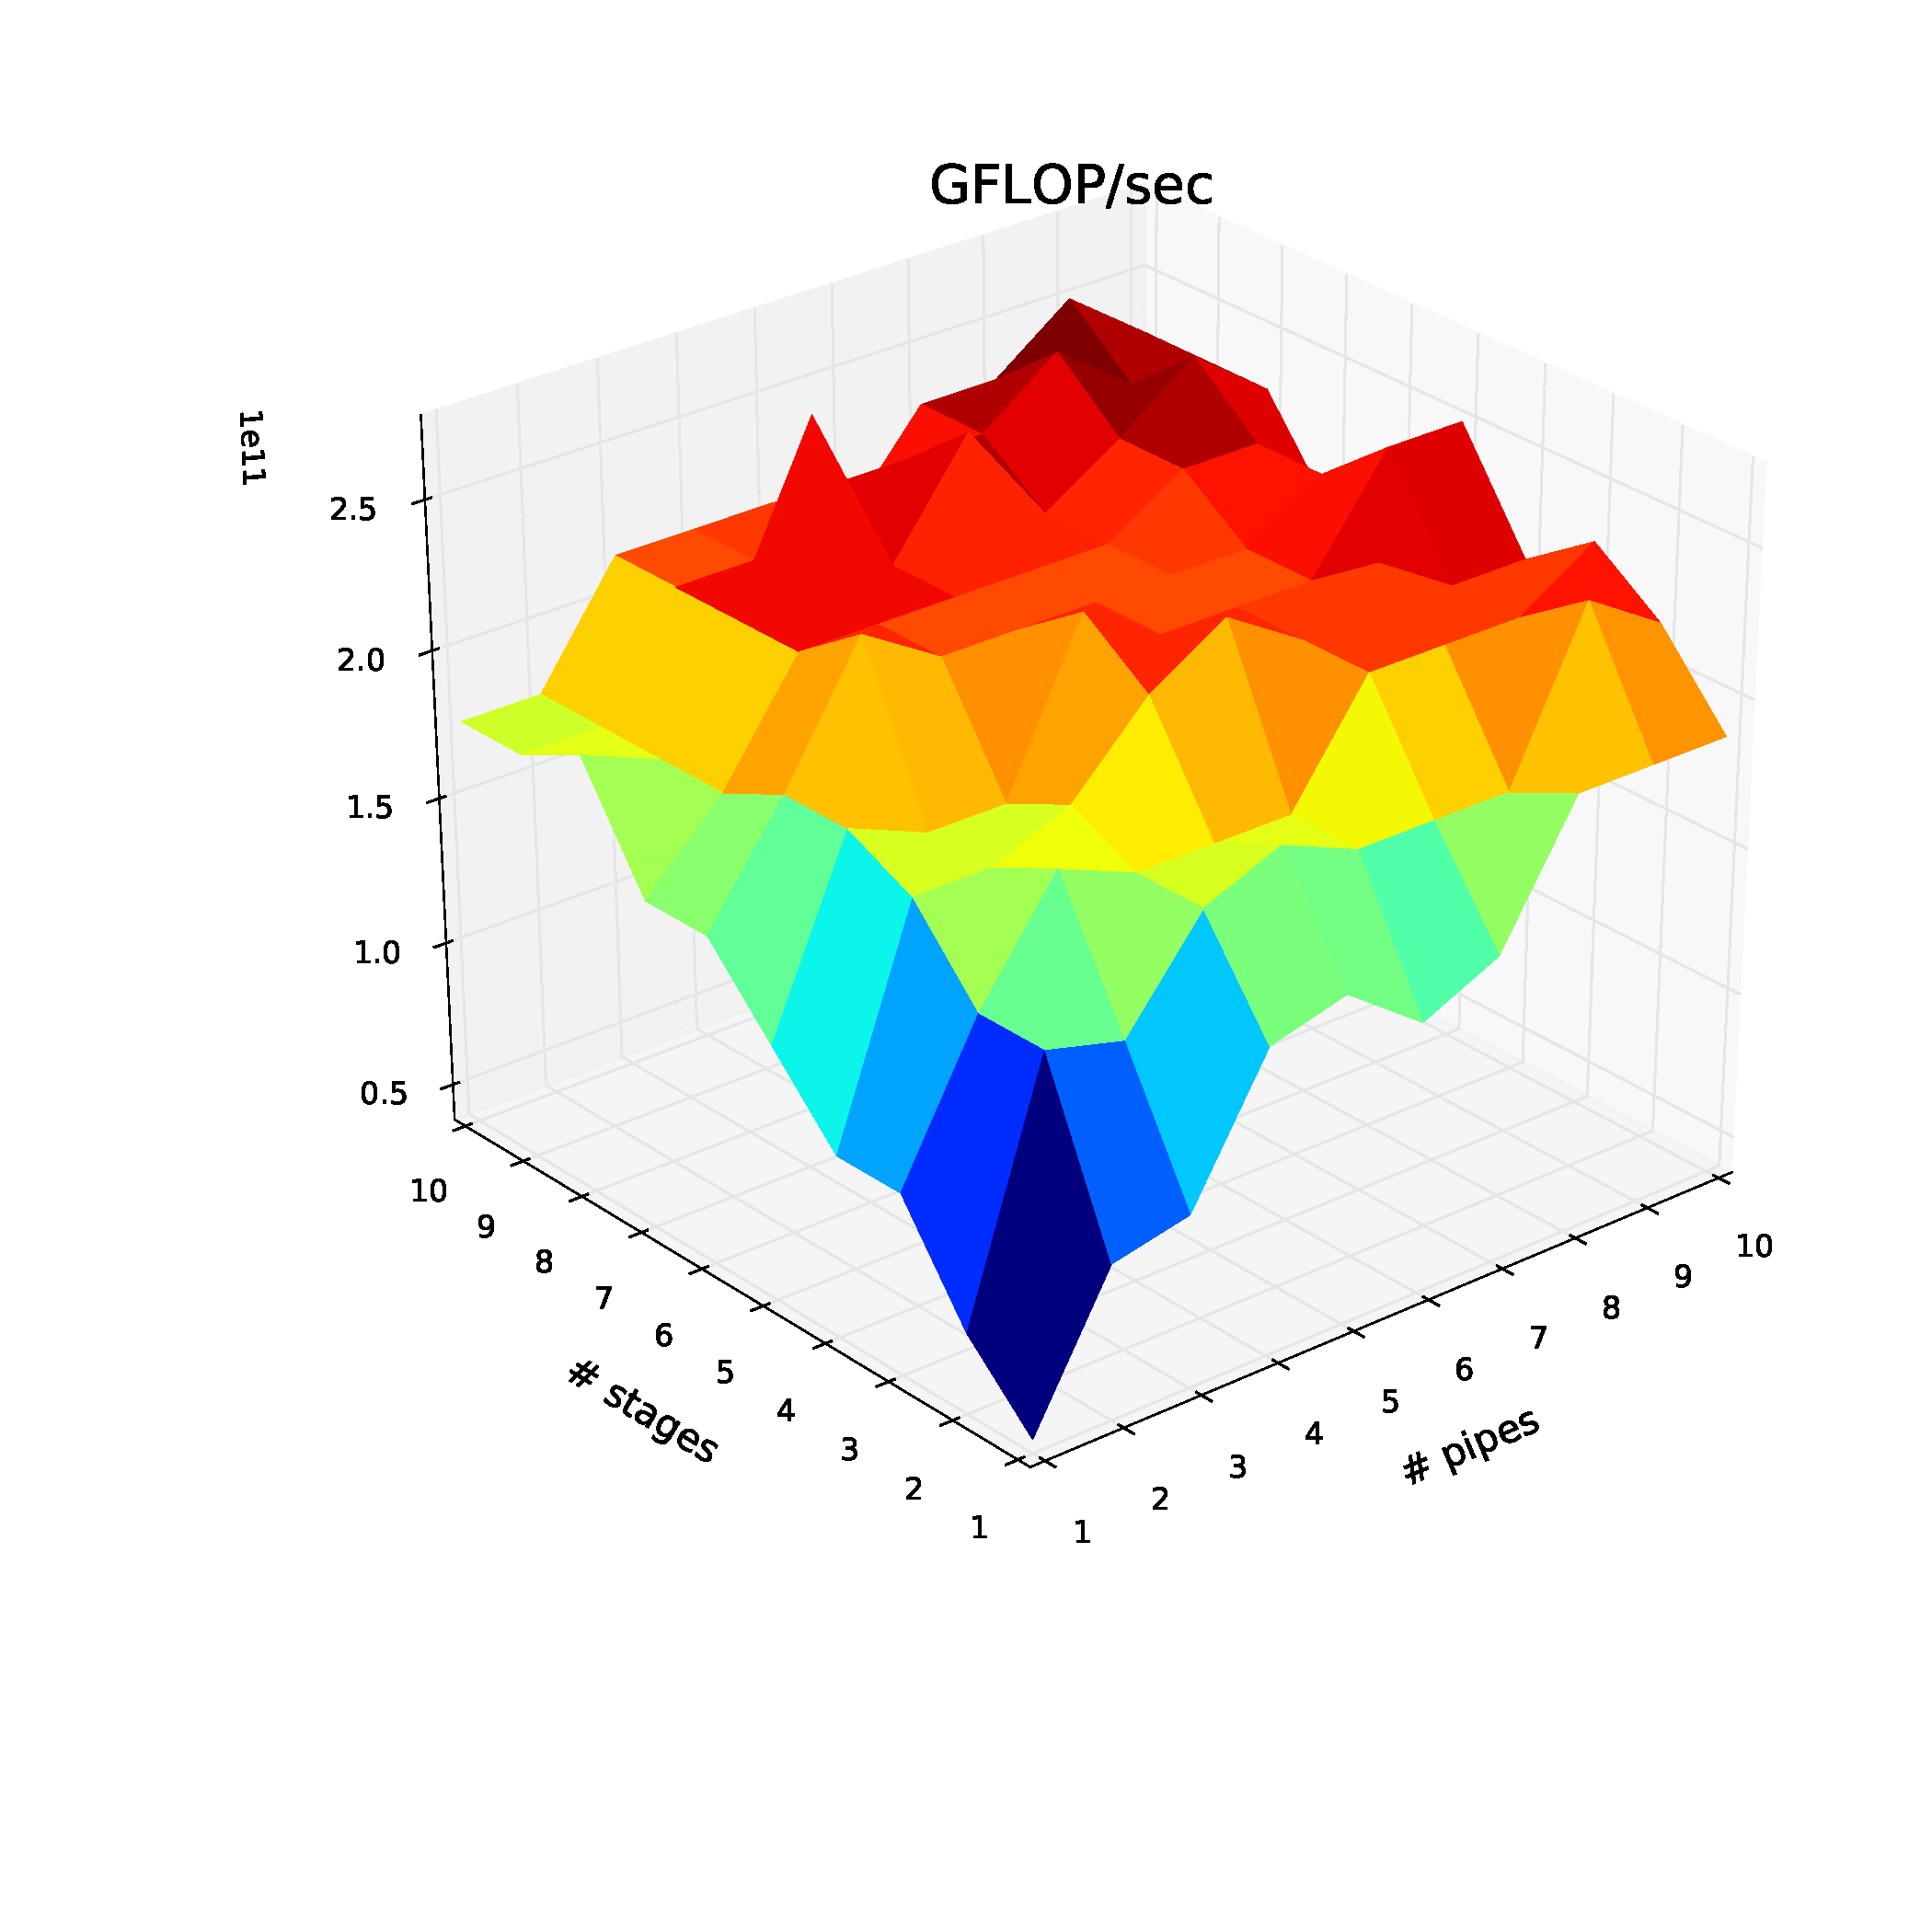
\includegraphics[width=\columnwidth]{fft_i7_generic.pdf}
    \caption{GFLOPs per second through an FFT array on an Intel i7.}
    \label{fig:fft_generic}
\end{figure}

\begin{figure}[htbp]
    \centering
    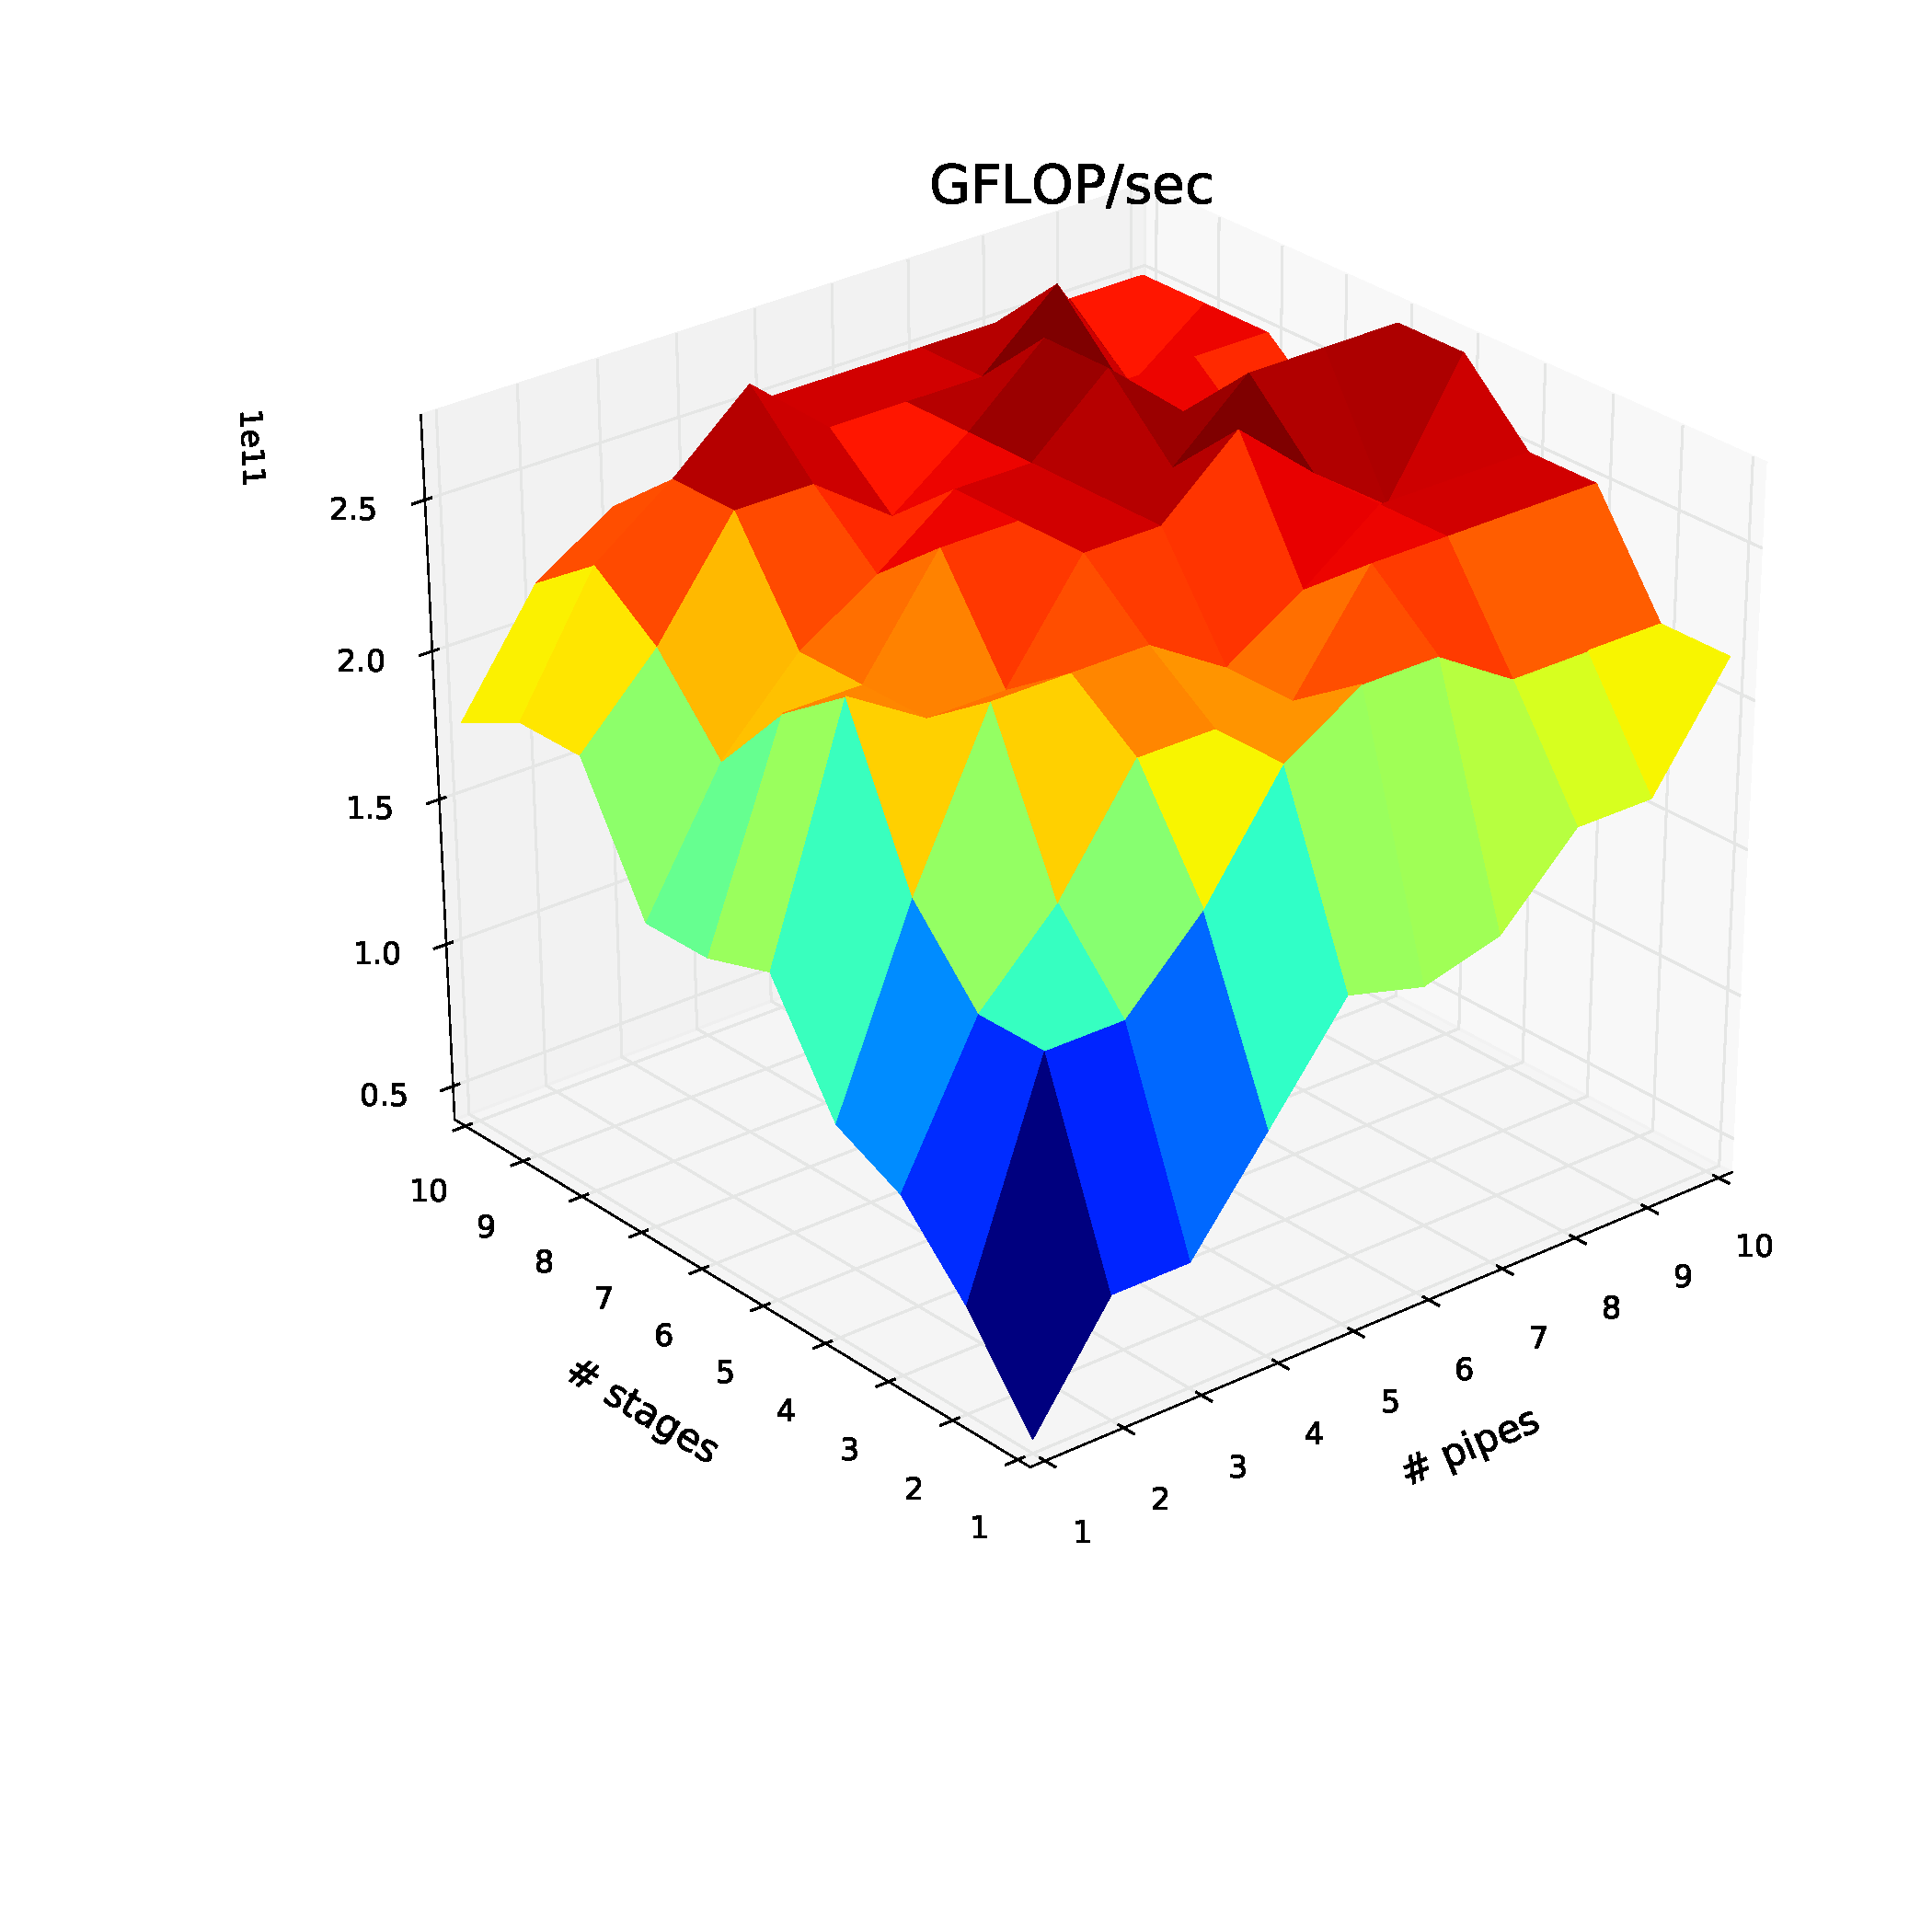
\includegraphics[width=\columnwidth]{fft_i7_volked.pdf}
    \caption{GFLOPs per second through an FFT array with VOLK enabled on an Intel i7.}
    \label{fig:fft_volk}
\end{figure}

Example output from multi-processor scheduling tests on an Intel i7 are shown in Figures \ref{fig:fft_generic}, \ref{fig:fft_volk}, \ref{fig:fir_generic}, \ref{fig:fir_volk}. 
The big performance differences come from using VOLK while doing parallel FFTs. 
On the FFT plots, Figures \ref{fig:fft_generic} and \ref{fig:fft_volk}, comparing the gradient in the direction of pipes verses stages yields an interesting difference between generic kernels and using VOLK.
Using generic kernels adding stages causes a larger increase to FLOPs/s compared to adding pipes; in contrast with VOLK enabled adding pipes causes an equivalent increase in FLOPs/s as adding stages does. 
Every processor will have a peak in the measured FLOPs where adding more pipes and stages will not yield an increase in FLOPs and past which the measured FLOPs will decrease, likely due to the increased need to store and fetch samples from memory. 

The FIR filter results do not seem affected by VOLK kernels being used as opposed to the generic kernels. 
This is likely because FIR filter blocks have already been hand-tuned to use SIMD instructions without VOLK \cite{gnu-list}. 

\begin{figure}[htbp]
    \centering
    \includegraphics[width=\columnwidth]{fir_i7_generic.pdf}
    \caption{GFLOPs per second through an FIR filter array on an Intel i7.}
    \label{fig:fir_generic}
\end{figure}

\begin{figure}[htbp]
    \centering
    \includegraphics[width=\columnwidth]{fir_i7_volked.pdf}
    \caption{GFLOPs per second through an FIR filter array with VOLK enabled on an Intel i7.}
    \label{fig:fir_volk}
\end{figure}




\subsection{VOLK kernels}

Figures \ref{fig:math_generic_compare} and \ref{fig:math_volk_compare} show the results of benchmarking VOLK math operations implemented as stand-alone GNU Radio blocks using generic kernels and with VOLK optimizations, respectively.
Type conversions with generic and VOLK improvements are shown in Figures \ref{fig:type_generic_compare} and \ref{fig:type_volk_compare}. 
The height of each bar in these four graphs is the total time to repeat the named operation 1 billion times; the black bar shows one standard deviation of those 1 billion measurements.
In each graph the \texttt{gr353} refers to GNU Radio version 3.5.3; \texttt{generic} or \texttt{volked} refers to either the generic proto-kernel implementation, or the optimized implementation as selected by \texttt{volk\_profile}; \texttt{atom} refers to the Intel Atom D525, \texttt{i7} refers to the Intel i7-980, \texttt{e110} refers to the Ettus E110 (TI OMAP 3730), \texttt{e350} refers to the AMD E350 APU, and \texttt{zc702} refers to the Xilinx ZC702 development board (XC7Z020).
For example, \texttt{i7\_gr353\_volked} refers to the Intel i7-980, with GNURadio v3.5.3, using the optimized VOLK proto-kernels.

\begin{figure}[htbp]
    \centering
    \includegraphics[width=\columnwidth]{math_generic_compare.pdf}
    \caption{VOLK math results using a generic VOLK kernel for different processors.}
    \label{fig:math_generic_compare}
\end{figure}

\begin{figure}[htbp]
    \centering
    \includegraphics[width=\columnwidth]{math_volked_compare.pdf}
    \caption{VOLK math results using VOLK kernels for different processors.}
    \label{fig:math_volk_compare}
\end{figure}

The Intel i7 is obviously much faster than other processors, and the E110 is obviously much slower. 
The E110 sees no improvement from VOLK across all benchmarks because ARM processors use the NEON architecture that is not well supported in VOLK yet.
Some highlights from the VOLK results are that nearly all instructions on the x86 processors do see improvement from generic kernels. 
It is also clear that some processors have more performance gain from VOLK than others. 
For example comparing the multiply\_cc, which executes a complex multiply and outputs a complex result, in Figure \ref{fig:math_generic_compare} the Atom is clearly faster than the E350 using generic kernels.
Using VOLK, Figure \ref{fig:math_volk_compare} shows that the E350 is now slightly faster than the Atom. 
Similar results appear Figures \ref{fig:math_generic_compare} and \ref{fig:math_volk_compare} with multiply\_conjugate\_cc, complex\_to\_mag in Figures \ref{fig:type_generic_compare} and \ref{fig:type_volk_compare}. 

\begin{figure}[htbp]
    \centering
    \includegraphics[width=\columnwidth]{types_generic_compare.pdf}
    \caption{VOLK type conversion results using a generic VOLK kernel for different processors.}
    \label{fig:type_generic_compare}
\end{figure}

\begin{figure}[htbp]
    \centering
    \includegraphics[width=\columnwidth]{types_volked_compare.pdf}
    \caption{VOLK type conversion results using VOLK kernels for different processors.}
    \label{fig:type_volk_compare}
\end{figure}

Some VOLK kernels are actually on par with or slower than the generic kernels. 
Since this occurs mostly on the simpler instructions such as add\_ff and multiply\_const\_ff the likely cause is compilers and processors are already fine-tuned to do these instructions efficiently. 

\section{Conclusion}
Multi-processor scheduling and speed of vector math will play an important role in processor selection for a software radio application. 
Being able to pick a processor that matches size, weight, and power constraints that match desired specifications requires knowledge of processor performance. 
By integrating and enhancing existing tools and working through the bugs to run GNU Radio through a Poky distribution build of OE we have introduced a benchmarking platform which can assist in choosing the best platform for embedded software radios.
We have also introduced benchmarking results for a small set of potentially suitable processors for software radio.
% \nocite{*} % this will include all citations

\bibliography{benchmarking_paper.bib}{}
\bibliographystyle{plain}

% \lstinputlisting[language=]{filename}
\lstset{numbers=left, basicstyle=\footnotesize\ttfamily, numberstyle=\tiny, stepnumber=4, numbersep=5pt,
title=\lstname, tabsize=5
}

\lstinputlisting[language=bash, breaklines, caption={Benchmark control script.}]{../run_benchmarking}
\lstinputlisting[language=Python, breaklines, caption={Modified helper functions for testing.}]{../utils/common_test_funcs.py}
\lstinputlisting[language=Python, breaklines, caption={Modified MatPlotLib for VOLK results plotting.}]{../volk/volk_plot.py}
\lstinputlisting[language=Python, breaklines, caption={MatPlotLib plotting tools for mp-sched results.}]{../mp-sched/mp_plot.py}
\lstinputlisting[language=Python, breaklines, caption={Modified mp-sched testing for FFTs}]{../mp-sched/run_synthetic_fft.py}

\end{document}
